\documentclass[10pt]{article}
% Formato extenso: report
\begin{sloppypar}
	
\end{sloppypar}
% Formato corto: article

% Esto es para que el LaTeX sepa que el texto está en español:
\usepackage[english]{babel}

\usepackage{amsmath, amsthm, amsfonts,amssymb}

% Bórrame si quieres:
\usepackage{multicol}

% Referencias
\usepackage{hyperref}

% Paquete para escribir código
\usepackage{listings}
\lstset{basicstyle=\footnotesize\ttfamily,breaklines=true}
\usepackage{alltt}

% Paquete para incluir imágenes
\usepackage{graphicx}

% Paquete para incluir varias imágenes en una
\usepackage{subfig}

% para poder fijar las imágenes ([H])
\usepackage{float}

% para agregar opciones al enumerate
\usepackage{enumerate}

% Teoremas
\newtheorem{thm}{Teorema}[section]
\newtheorem{cor}[thm]{Corolario}
\newtheorem{lem}[thm]{Lema}
\newtheorem{prop}[thm]{Proposición}
\theoremstyle{definition}
\newtheorem{defn}[thm]{Definición}
\theoremstyle{remark}
\newtheorem{rem}[thm]{Observación}
\theoremstyle{definition}
\newtheorem{prob}{Problema}
\numberwithin{equation}{prob}

% Calculus symbols
\newcommand{\pd}[2]{\frac{\partial #1}{ \partial #2}}   % First partial derivative command
\newcommand{\td}[2]{\frac{\mathrm{d} #1}{ \mathrm{d} #2}}
\newcommand{\pdd}[2]{\frac{\partial^2 #1}{ \partial #2 ^2}}   % Second partial derivative command
\newcommand{\pddc}[3]{\frac{\partial^2 #1}{ \partial #2 \partial #3}}   % Second partial derivative command

% Continuum mechanics & FEM symbols
\def\sca   #1{\mbox{\rm{#1}}{}}
\def\mat   #1{\mbox{\boldmath $\mathsf #1$}}
\def\vec   #1{\mbox{\boldmath $#1$}{}}
\def\ten   #1{\mbox{\boldmath $#1$}{}}
\def\ltr   #1{\mbox{\sf{#1}}}
\def\bltr  #1{\mbox{\sffamily{\bfseries{{#1}}}}}

% math operators and symbols
\DeclareMathOperator{\dive}{div}
\DeclareMathOperator{\trace}{trace}
\DeclareMathOperator{\tr}{tr}
\DeclareMathOperator{\symm}{symm}
\DeclareMathOperator{\sk}{skew}
\DeclareMathOperator{\grad}{grad}
\DeclareMathOperator{\Grad}{Grad}
\DeclareMathOperator{\curl}{curl}
\DeclareMathOperator{\Curl}{Curl}
\def\R{\mbox{\(\mathbb{R}\)}}
\def\dx{\mbox{\(\,\mathrm{d}x\)}}


\usepackage{geometry}
\geometry{left=2.5cm, right=2.5cm, top=2cm, bottom=3cm}

\usepackage{makeidx}
\makeindex


\begin{document}
	
	\begin{titlepage}
		
		
		%%%%% NO MODIFICAR
		\begin{figure}
			\begin{minipage}{4cm}
				
\includegraphics[width=0.9\textwidth]{./figures/logo}
			\end{minipage}
			\begin{minipage}{11cm}
				\vspace{4mm}
				{\sc UNIVERSIDAD DE VALPARAÍSO}\\
				Escuela de Ingeniería Civil Biomédica\\
				{\bf CBM414 Procesamiento digital de señales biomédicas}\\
				\vspace{0mm}
				\hrulefill
			\end{minipage}
		\end{figure}
		\phantom{""}\vspace{60mm}
		
		
		%%%%% MODIFICAR
		\begin{center}
			\Huge{\textbf{Laboratory 3}}\vspace{95mm}\\
			\raggedleft \Large{Maximiliano Antonio Gaete Pizarro}\\ 
		\end{center}
		
		
	\end{titlepage}
	
\printindex


\section{Problem 1: Quantization of an Audio Signal}

\subsection{Explain in detail what the function \texttt{cuantizar} does.}

The function \texttt{cuantizar(s, bit)} quantizes an input signal \( s \) using a specified number of bits \( \text{bit} \). Below is a detailed explanation of each step:

\begin{lstlisting}[language=Python]
	def cuantizar(s,bit):
		# s: senal de entrada
        	# bit: bits de cuantificacion
		Plus1=np.power(2, (bit-1))
		X=s*Plus1
		X=np.round(X)
		X=np.minimum(Plus1-1.0,X)
		X=np.maximum(-1.0*Plus1,X)
		X=X/Plus1
		return X
		\end{lstlisting}

\begin{enumerate}
    \item \textbf{Calculate the Positive Quantization Levels:}

    \begin{lstlisting}[language=Python]
Plus1 = np.power(2, (bit - 1))
    \end{lstlisting}

    \textit{Explanation:} Computes \( 2^{(\text{bit} - 1)} \), which determines the number of positive quantization levels available. For instance, if \( \text{bit} = 4 \), then \( \text{Plus1} = 8 \).

    \item \textbf{Scale the Input Signal:}

    \begin{lstlisting}[language=Python]
X = s * Plus1
    \end{lstlisting}

    \textit{Explanation:} Scales the input signal \( s \) by multiplying it with \( \text{Plus1} \) to adjust it to the range of the quantization levels.

    \item \textbf{Round the Scaled Signal:}

    \begin{lstlisting}[language=Python]
X = np.round(X)
    \end{lstlisting}

    \textit{Explanation:} Rounds the values of \( X \) to the nearest integer, assigning each sample to the nearest quantization level.

    \item \textbf{Limit the Quantized Values to Prevent Saturation:}

    \begin{lstlisting}[language=Python]
X = np.minimum(Plus1 - 1.0, X)
X = np.maximum(-1.0 * Plus1, X)
    \end{lstlisting}

    \textit{Explanation:} Ensures that \( X \) does not exceed the maximum and minimum levels allowed by the number of bits. It constrains \( X \) within the range \([ -2^{(\text{bit} - 1)}, 2^{(\text{bit} - 1)} - 1 ]\).

    \item \textbf{Normalize the Quantized Signal:}

    \begin{lstlisting}[language=Python]
X = X / Plus1
return X
    \end{lstlisting}

    \textit{Explanation:} Normalizes the quantized signal by dividing by \( \text{Plus1} \), returning it to the original amplitude range.
\end{enumerate}

\textbf{Summary:} The function \texttt{cuantizar} scales the input signal, rounds the values to assign them to discrete quantization levels, limits the values to prevent saturation, and normalizes the quantized signal. This results in a quantized version of the original signal using the specified number of bits.

\subsection{Re-quantize the audio signal to 2, 4, and 8 bits. Listen to the signals and describe what you perceive.}

We re-quantize the normalized audio signal \texttt{x\_norm} using the \texttt{cuantizar} function:

\begin{lstlisting}[language=Python]
# Re-quantization of the signal to 2, 4, and 8 bits
xq_2bit = cuantizar(x_norm, 2)
xq_4bit = cuantizar(x_norm, 4)
xq_8bit = cuantizar(x_norm, 8)
\end{lstlisting}

\textbf{Perception after listening:}

\begin{itemize}
    \item \textbf{2 bits:} The audio sounds heavily distorted with significant quantization noise. Due to only 4 quantization levels, the signal loses most of its detail, and artifacts are prominent.
    \item \textbf{4 bits:} The audio quality improves but still contains noticeable distortion. With 16 quantization levels, the signal retains more detail, but quantization noise is still audible.
    \item \textbf{8 bits:} The audio closely resembles the original signal. With 256 quantization levels, the quantization noise is minimal, and the signal preserves much of the original quality.
\end{itemize}

\subsection{Plot the original and quantized signals for 2, 4, and 8 bits (three plots). What do you observe in the graphs?}

We plot a segment of the original signal and its quantized versions for visualization.

\begin{lstlisting}[language=Python]
# Define a segment of the signal for visualization
start_sample = 10000
end_sample = 10500

# Plot for 2 bits
plt.figure(figsize=(17, 4))
plt.plot(t[start_sample:end_sample], x_norm[start_sample:end_sample], label='Original')
plt.step(t[start_sample:end_sample], xq_2bit[start_sample:end_sample], label='Quantized (2 bits)', where='mid', alpha=0.7)
plt.title('Original vs. Quantized Signal (2 bits)')
plt.xlabel('Time [s]')
plt.ylabel('Amplitude')
plt.legend()
plt.grid()
plt.show()

# Plot for 4 bits
plt.figure(figsize=(17, 4))
plt.plot(t[start_sample:end_sample], x_norm[start_sample:end_sample], label='Original')
plt.step(t[start_sample:end_sample], xq_4bit[start_sample:end_sample], label='Quantized (4 bits)', where='mid', alpha=0.7)
plt.title('Original vs. Quantized Signal (4 bits)')
plt.xlabel('Time [s]')
plt.ylabel('Amplitude')
plt.legend()
plt.grid()
plt.show()

# Plot for 8 bits
plt.figure(figsize=(17, 4))
plt.plot(t[start_sample:end_sample], x_norm[start_sample:end_sample], label='Original')
plt.step(t[start_sample:end_sample], xq_8bit[start_sample:end_sample], label='Quantized (8 bits)', where='mid', alpha=0.7)
plt.title('Original vs. Quantized Signal (8 bits)')
plt.xlabel('Time [s]')
plt.ylabel('Amplitude')
plt.legend()
plt.grid()
plt.show()
\end{lstlisting}

\begin{itemize}
    \item \textbf{For 2 bits:}

    \begin{figure}[H]
    \centering
    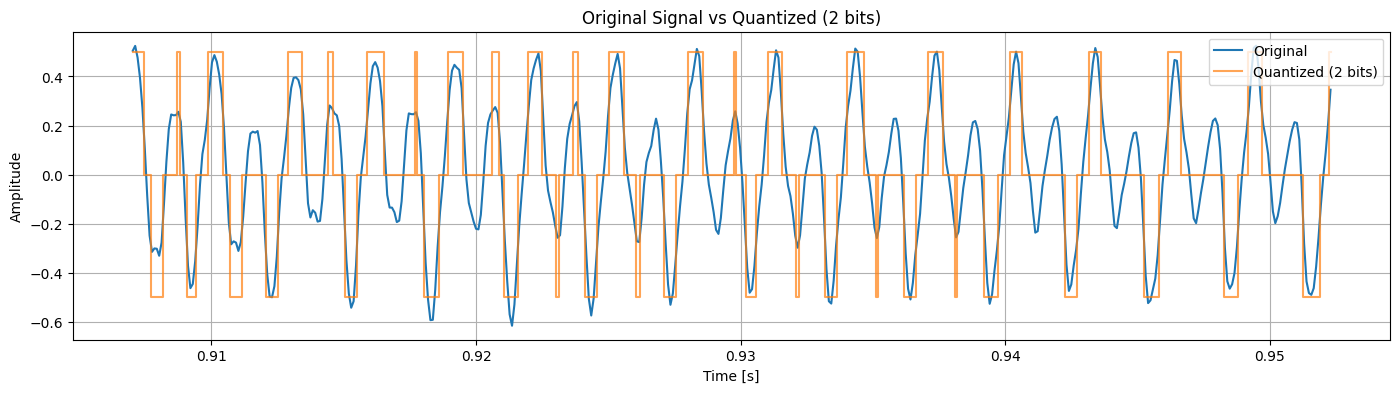
\includegraphics[width=1\textwidth]{./figures/original_vs_quantized_2bits.png}
    \caption{Original vs. Quantized Signal (2 bits)}
    \end{figure}

    \item \textbf{For 4 bits:}

    \begin{figure}[H]
    \centering
    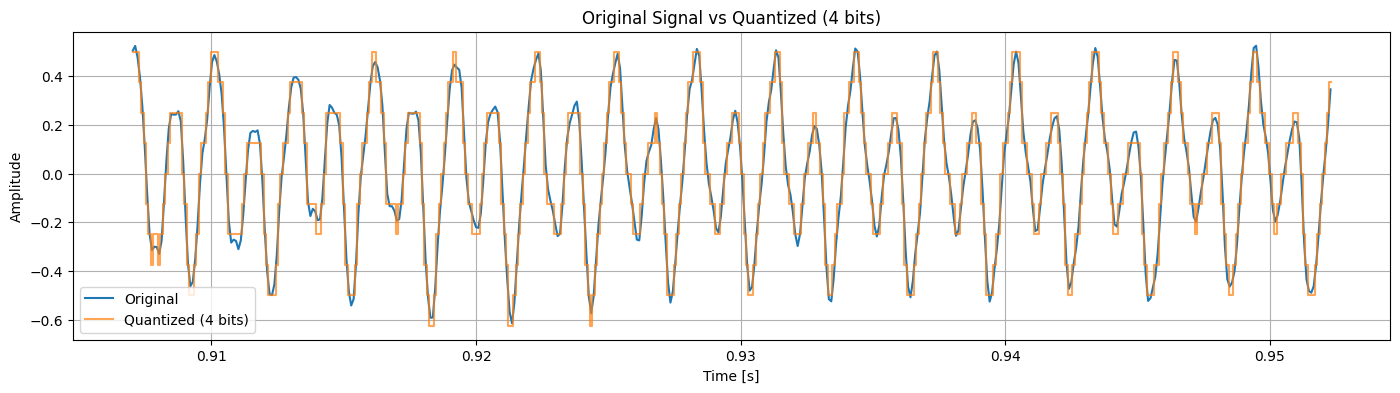
\includegraphics[width=1\textwidth]{./figures/original_vs_quantized_4bits.png}
    \caption{Original vs. Quantized Signal (4 bits)}
    \end{figure}

    \item \textbf{For 8 bits:}

    \begin{figure}[H]
    \centering
    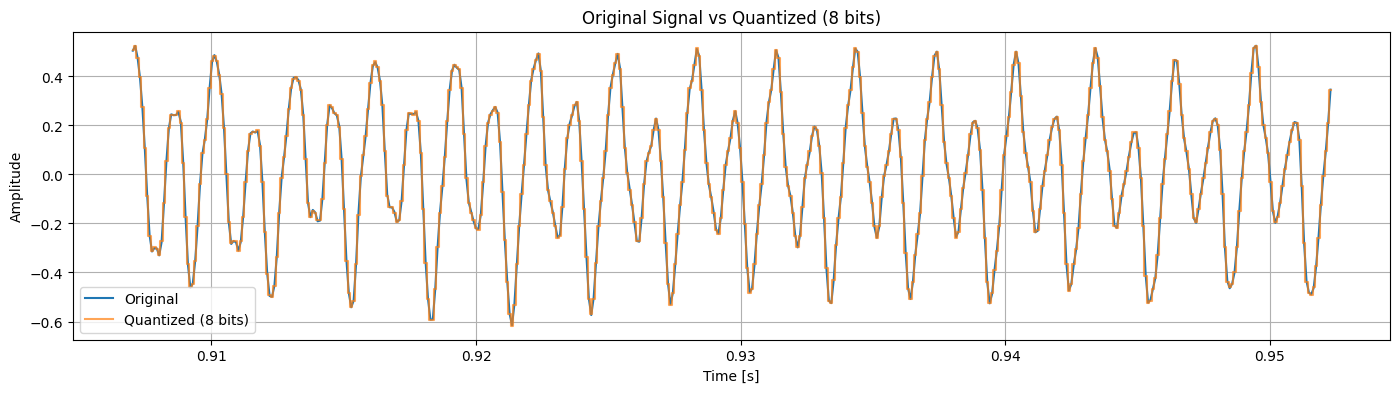
\includegraphics[width=1\textwidth]{./figures/original_vs_quantized_8bits.png}
    \caption{Original vs. Quantized Signal (8 bits)}
    \end{figure}
\end{itemize}

\textbf{Observations:}

\begin{itemize}
    \item \textbf{2 bits:} The quantized signal approximates the original signal with very coarse steps, resulting in a blocky waveform. The lack of levels causes a poor representation of the signal.
    \item \textbf{4 bits:} The quantization steps are finer compared to the 2-bit case. The quantized signal follows the original more closely but still shows noticeable stepping.
    \item \textbf{8 bits:} The quantized signal closely matches the original waveform. The steps are so fine that they are hardly noticeable, indicating a high-quality quantization.
\end{itemize}

\subsection{Calculate the quantization error (RMS) for 2, 4, and 8 bits. What can you conclude from the results?}

We calculate the Root Mean Square (RMS) error using the \texttt{rms} function:

\begin{lstlisting}[language=Python]
# Calculation of the RMS error
error_2bit = rms(x_norm, xq_2bit)
error_4bit = rms(x_norm, xq_4bit)
error_8bit = rms(x_norm, xq_8bit)

print(f"RMS Error for 2 bits: {error_2bit}")
print(f"RMS Error for 4 bits: {error_4bit}")
print(f"RMS Error for 8 bits: {error_8bit}")
\end{lstlisting}

\textbf{Computed RMS Errors:}

\begin{itemize}
    \item \textbf{2 bits:} \( \text{Error}_{\text{RMS}}^{(2\,\text{bits})} = 0.1411 \)
    \item \textbf{4 bits:} \( \text{Error}_{\text{RMS}}^{(4\,\text{bits})} = 0.0358 \)
    \item \textbf{8 bits:} \( \text{Error}_{\text{RMS}}^{(8\,\text{bits})} = 0.0022 \)
\end{itemize}


\textbf{Conclusions:}

\begin{itemize}
    \item The RMS error decreases significantly as the number of bits increases.
    \item Increasing the bit depth reduces quantization error, leading to a more accurate representation of the original signal.
    \item There is a substantial improvement in error reduction from 2 bits to 4 bits, and from 4 bits to 8 bits, indicating the importance of bit depth in quantization.
\end{itemize}

\subsection{Plot the difference (point by point) between the original and re-quantized signals for 2, 4, and 8 bits (single plot). What can you conclude from the above graph?}

We compute the differences and plot them:

\begin{lstlisting}[language=Python]
# Calculation of the differences
diff_2bit = x_norm - xq_2bit
diff_4bit = x_norm - xq_4bit
diff_8bit = x_norm - xq_8bit

# Plotting the quantization errors
plt.figure(figsize=(20, 6))
plt.plot(t[start_sample:end_sample], diff_2bit[start_sample:end_sample], label='Error (2 bits)')
plt.plot(t[start_sample:end_sample], diff_4bit[start_sample:end_sample], label='Error (4 bits)')
plt.plot(t[start_sample:end_sample], diff_8bit[start_sample:end_sample], label='Error (8 bits)')
plt.title('Quantization Error for 2, 4, and 8 bits')
plt.xlabel('Time [s]')
plt.ylabel('Amplitude Difference')
plt.legend()
plt.grid()
plt.show()
\end{lstlisting}

\begin{figure}[H]
\centering
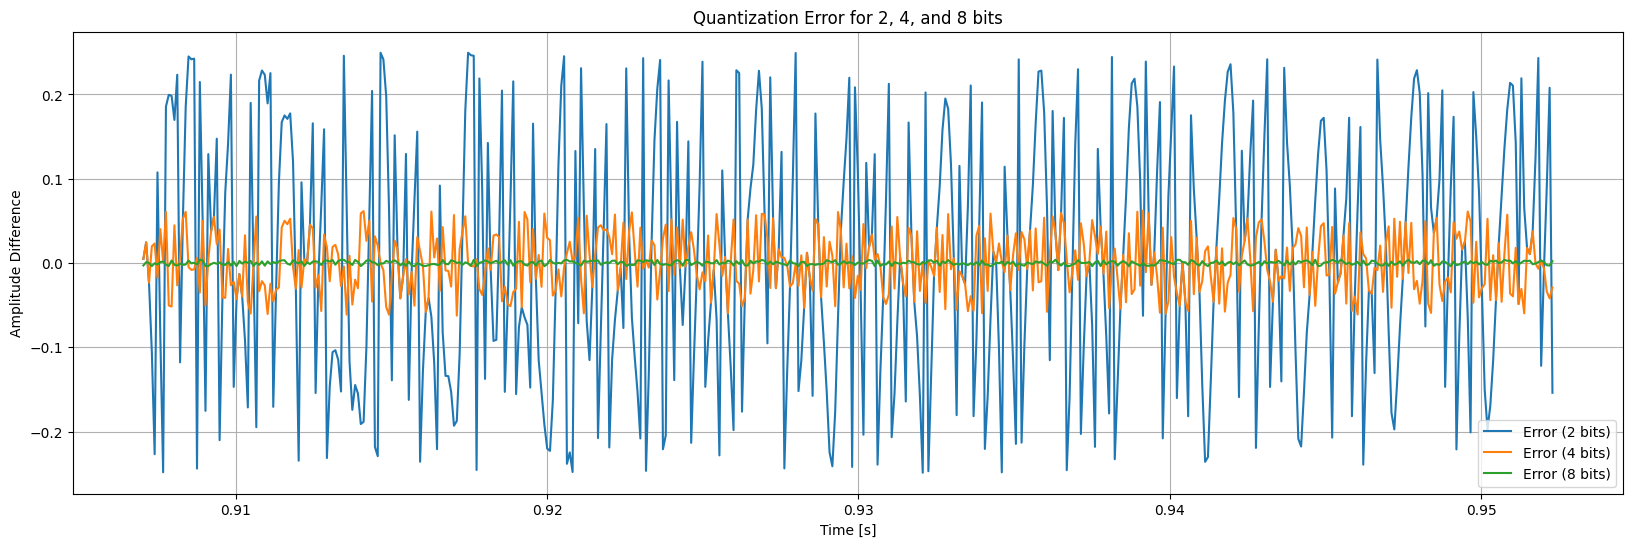
\includegraphics[width=1\textwidth]{./figures/quantization_error.png}
\caption{Quantization Error for 2, 4, and 8 bits}
\end{figure}

\textbf{Conclusions:}

\begin{itemize}
    \item \textbf{Error Magnitude:} The magnitude of the quantization error decreases with increasing bit depth.
    \item \textbf{2 bits:} Shows large error values, indicating significant distortion and loss of information.
    \item \textbf{4 bits:} Error values are smaller but still noticeable, reflecting moderate quantization noise.
    \item \textbf{8 bits:} Error values are minimal, indicating that the quantized signal closely approximates the original signal.
    \item \textbf{Pattern of Errors:} The error signals resemble random noise superimposed on the signal, characteristic of quantization noise.
\end{itemize}

\textbf{Overall Conclusions:}

\begin{itemize}
    \item \textbf{Impact of Bit Depth:} Increasing the number of quantization bits greatly improves the quality of the quantized signal by reducing quantization error.
    \item \textbf{Quantization Noise:} Quantization introduces noise that can be perceived in the audio signal, especially at lower bit depths.
    \item \textbf{Optimal Bit Depth:} There is a trade-off between the number of bits (which affects data size and processing requirements) and the quality of the quantized signal. Selecting an appropriate bit depth depends on the application's requirements for quality and resources.
\end{itemize}

\section{Problem 2: Noise in an Audio Signal}

\subsection{Briefly explain what the function \texttt{add\_gaussian\_noise} does. Use the definition of \( SNR_{dB} \) to explain, step by step mathematically, how the variable \texttt{noise\_variance} was derived within the function.}

Code for \texttt{add\_gaussian\_noise} and \texttt{calculate\_snr}

\begin{lstlisting}[language=Python]
def add_gaussian_noise(signal, snr_db):

    # Calculate the signal power
    signal_power = np.mean(signal**2)

    # Calculate the desired noise power
    snr_linear = 10**(snr_db / 10)
    noise_power = signal_power / snr_linear

    # Calculate the noise variance
    noise_variance = noise_power

    # Generate Gaussian noise
    noise = np.sqrt(noise_variance) * np.random.randn(*signal.shape)

    # Add the noise to the signal
    noisy_signal = signal + noise

    return noisy_signal, noise

def calculate_snr(signal, noise):
    """ Calculates the SNR between an input signal "signal" and noise "noise" """
    # Ensure numpy arrays
    signal, noise = np.array(signal), np.array(noise)

    # Calculate the power of the signal and the noise
    signal_power = np.mean(signal**2)
    noise_power = np.mean(noise**2)

    # Calculate the SNR in decibels (dB)
    snr = 10 * np.log10(signal_power / noise_power)
    return snr
\end{lstlisting}

\textbf{Explanation of the \texttt{add\_gaussian\_noise} Function:}

The function \texttt{add\_gaussian\_noise} adds Gaussian noise to a signal to achieve a specified Signal-to-Noise Ratio (SNR) in decibels (dB). Below is a step-by-step mathematical explanation of how the variable \texttt{noise\_variance} is derived.

\textbf{Step 1: Calculate the Signal Power \( E[S^2] \)}

\[
\text{signal\_power} = E[S^2] = \frac{1}{N} \sum_{n=1}^{N} s[n]^2
\]

This computes the average power of the signal.

\textbf{Step 2: Convert SNR from dB to Linear Scale}

\[
\text{snr\_linear} = 10^{(\text{snr\_db} / 10)}
\]

This step converts the desired SNR from decibels to a linear scale.

\textbf{Step 3: Calculate the Desired Noise Power \( E[N^2] \)}

Using the definition of SNR in linear terms:

\[
\text{SNR}_{\text{linear}} = \frac{E[S^2]}{E[N^2]}
\]

Solving for \( E[N^2] \):

\[
E[N^2] = \frac{E[S^2]}{\text{SNR}_{\text{linear}}}
\]

Therefore:

\[
\text{noise\_power} = \frac{\text{signal\_power}}{\text{snr\_linear}}
\]

\textbf{Step 4: Calculate the Noise Variance}

For zero-mean Gaussian noise, the variance equals the power:

\[
\text{noise\_variance} = \text{noise\_power}
\]

\textbf{Step 5: Generate Gaussian Noise}

\[
\text{noise} = \sqrt{\text{noise\_variance}} \times \text{randn}(N)
\]

Where \(\text{randn}(N)\) generates \( N \) samples of standard normal random variables.

\textbf{Step 6: Add the Noise to the Signal}

\[
\text{noisy\_signal} = \text{signal} + \text{noise}
\]

Thus, the variable \texttt{noise\_variance} is derived to ensure that the added Gaussian noise results in the desired SNR.

\subsection{Contaminate the audio signal with Gaussian noise using the function \texttt{noise = np.random.normal(0, var, len(signal))}, where \( \text{Var} = 0.1, 0.01, 0.001 \). Listen to the signals and briefly describe what you perceive.}

Code for Adding Gaussian Noise with Specified Variance

\begin{lstlisting}[language=Python]
# Variances to use
variances = [0.1, 0.01, 0.001]

# Contaminate the signal and listen
for var in variances:
    # Generate Gaussian noise
    noise = np.random.normal(0, np.sqrt(var), len(x_norm))
    
    # Noisy signal
    noisy_signal = x_norm + noise
    
    # Listen to the signal
    print(f"Signal with Gaussian noise of variance {var}:")
    display(Audio(noisy_signal, rate=fs))
\end{lstlisting}

\textbf{Perceptions after Listening:}

\begin{itemize}
    \item \textbf{Variance \( = 0.1 \):} The noise is very prominent, significantly distorting the original audio signal. The speech or music becomes difficult to understand due to the high level of noise.
    \item \textbf{Variance \( = 0.01 \):} The noise is noticeable but less intrusive. The original audio can still be heard, but the quality is degraded.
    \item \textbf{Variance \( = 0.001 \):} The noise is minimal, and the audio quality is close to the original. Any noise present is barely perceptible.
\end{itemize}

\subsection{Calculate the \( SNR_{dB} \) using the function \texttt{calculate\_snr} and report the values for the three given variances. Does \( SNR_{dB} \) increase, decrease, or stay the same? What can you conclude from the results, emphasizing the meaning of decibels?}

Code for Calculating SNR

\begin{lstlisting}[language=Python]
# List to store the calculated SNRs
snr_values = []

# Original signal power
signal_power = np.mean(x_norm**2)

for var in variances:
    # Generate Gaussian noise
    noise = np.random.normal(0, np.sqrt(var), len(x_norm))
    
    # Noisy signal
    noisy_signal = x_norm + noise
    
    # Calculate the SNR
    snr = calculate_snr(x_norm, noise)
    snr_values.append(snr)
    
    print(f"SNR_dB for variance {var}: {snr:.2f} dB")
\end{lstlisting}

\textbf{Calculated \( SNR_{dB} \) Values:}

\begin{itemize}
    \item \textbf{Variance \( = 0.1 \):} \( SNR_{dB} \approx -3.09 \) dB
    \item \textbf{Variance \( = 0.01 \):} \( SNR_{dB} \approx 6.87 \) dB
    \item \textbf{Variance \( = 0.001 \):} \( SNR_{dB} \approx 16.91 \) dB
\end{itemize}

\textbf{Conclusions:}

\begin{itemize}
    \item As the variance decreases from 0.1 to 0.001, the \( SNR_{dB} \) increases.
    \item A lower noise variance means less noise power, resulting in a higher SNR.
    \item The increase in \( SNR_{dB} \) is logarithmic due to the decibel scale. Each 10-fold decrease in noise power results in a 10 dB increase in SNR.
    \item Decibels provide a logarithmic measure of the ratio between signal and noise power, making it easier to represent large variations in power ratios.
\end{itemize}

\subsection{Use the function \texttt{add\_gaussian\_noise} and add Gaussian noise with \( SNR_{dB} = 1, 10, 30 \). Use the second output of the function, i.e., \texttt{noise}, and calculate the variance. What can you conclude from the results?}

Code for Adding Noise and Calculating Variance

\begin{lstlisting}[language=Python]
# SNR_dB values to use
snr_db_values = [1, 10, 30]

# List to store the calculated variances
noise_variances = []

for snr_db in snr_db_values:
    # Add Gaussian noise with the specified SNR_dB
    noisy_signal, noise = add_gaussian_noise(x_norm, snr_db)
    
    # Calculate the variance of the noise
    noise_variance = np.var(noise)
    noise_variances.append(noise_variance)
    
    print(f"For SNR_dB = {snr_db}:")
    print(f"Noise variance = {noise_variance:.6f}\n")
\end{lstlisting}

\textbf{Calculated Noise Variances:}

\begin{itemize}
    \item \textbf{\( SNR_{dB} = 1 \):} Noise variance \( \approx 0.039517 \)
    \item \textbf{\( SNR_{dB} = 10 \):} Noise variance \( \approx 0.004969 \)
    \item \textbf{\( SNR_{dB} = 30 \):} Noise variance \( \approx 0.000049 \)
\end{itemize}

\textbf{Conclusions:}

\begin{itemize}
    \item As \( SNR_{dB} \) increases, the calculated noise variance decreases.
    \item A higher \( SNR_{dB} \) implies a higher signal-to-noise ratio, which requires a lower noise power (variance).
    \item The relationship between \( SNR_{dB} \) and noise variance is logarithmic. Each 10 dB increase in SNR corresponds to a 10-fold decrease in noise variance.
    \item These results confirm that to achieve a higher SNR, the noise added to the signal must have a lower variance.
\end{itemize}

\subsection{Overall Conclusions}

\begin{itemize}
    \item The functions \texttt{add\_gaussian\_noise} and \texttt{calculate\_snr} are consistent with the mathematical definitions of signal power, noise power, and SNR.
    \item Adding Gaussian noise with specified variances affects the perceptual quality of the audio signal, with higher variances leading to more audible noise.
    \item The \( SNR_{dB} \) is inversely related to the noise variance; decreasing noise variance increases \( SNR_{dB} \).
    \item Understanding the relationship between SNR, noise variance, and their impact on signal quality is crucial in signal processing applications.
\end{itemize}

\section{Problem 3: Noise in an ECG Signal}

\subsection{Plot the signal without noise and with noise. Also, calculate the SNR in dB of the signal with respect to the noise that contaminates it.}

\subsubsection*{Code for Generating and Plotting the ECG Signals}

\begin{lstlisting}[language=Python]
# Parameters
sampling_rate = 200  # Sampling frequency in Hz
capture_length = 10  # Signal duration in seconds

def create_ECG_signal():
    bpm = 60  # Beats per minute
    bps = bpm / 60  # Beats per second

    # Create a wave similar to a heartbeat
    pqrst = signal.wavelets.daub(10)
    samples_rest = 10
    zero_array = np.zeros(samples_rest, dtype=float)
    pqrst_full = np.concatenate([pqrst, zero_array])

    # Concatenate the beats to cover the entire duration
    ecg_template = np.tile(pqrst_full, int(capture_length * bps))

    # Resample the signal to match the desired sampling frequency
    ecg_sampled = signal.resample(ecg_template, int(sampling_rate * capture_length))
    ecg_sampled = ecg_sampled / np.max(np.abs(ecg_sampled))  # Normalize
    ecg_sampled = 1.5 * ecg_sampled + 1  # Adjust amplitude and DC level

    return ecg_sampled

# Generate the ECG signal without noise
ecg_sampled = create_ECG_signal()

# Time vector
time = np.arange(0, capture_length, 1 / sampling_rate)

# Generate random noise and 50 Hz noise
np.random.seed(0)  # For reproducibility
noise = np.random.normal(0, 0.1, len(ecg_sampled))
noise50hz = 0.5 * np.sin(2 * np.pi * 50 * time)

# ECG signal with noise
ecg_noisy_sampled = ecg_sampled + noise + noise50hz

# Plot the signals
plt.figure(figsize=(12, 6))

plt.subplot(2, 1, 1)
plt.plot(time, ecg_sampled)
plt.title('ECG Signal without Noise')
plt.xlabel('Time [s]')
plt.ylabel('Amplitude')
plt.grid()

plt.subplot(2, 1, 2)
plt.plot(time, ecg_noisy_sampled, color='r')
plt.title('ECG Signal with Noise')
plt.xlabel('Time [s]')
plt.ylabel('Amplitude')
plt.grid()

plt.tight_layout()
plt.show()
\end{lstlisting}

\subsubsection*{Calculation of SNR}

\begin{lstlisting}[language=Python]
# Calculate the power of the signal and the noise
signal_power = np.mean(ecg_sampled ** 2)
noise_power = np.mean((noise + noise50hz) ** 2)

# Calculate the SNR in decibels
SNR_dB = 10 * np.log10(signal_power / noise_power)
print(f"The SNR of the signal with respect to the noise is: {SNR_dB:.2f} dB")
\end{lstlisting}

\subsubsection*{Results and Discussion}

\begin{figure}[H]
    \centering
    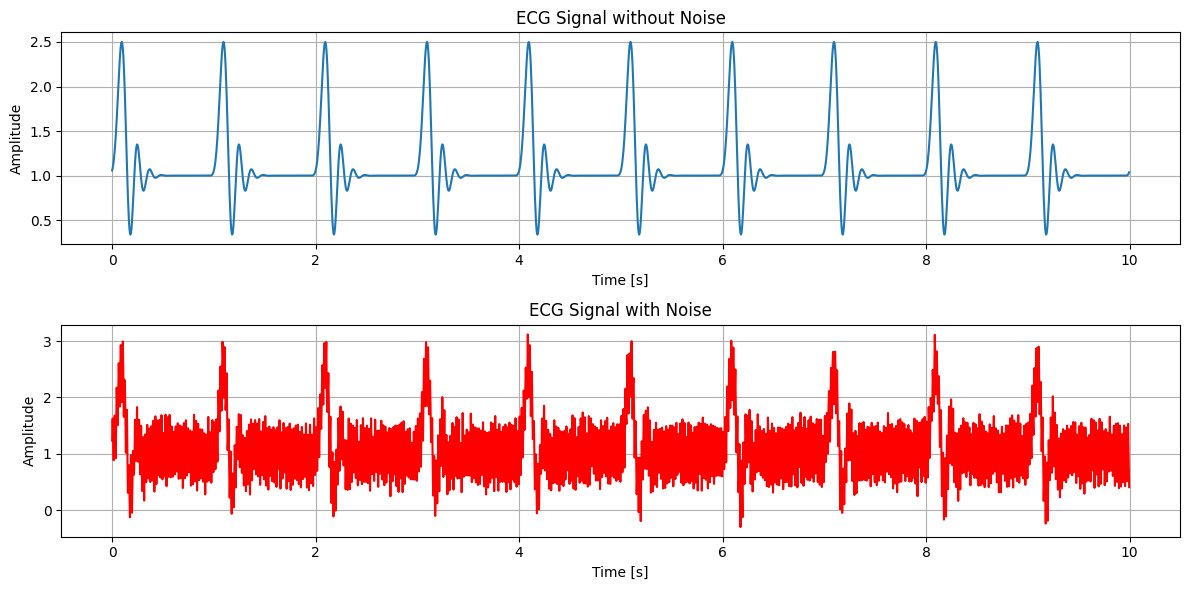
\includegraphics[width=0.9\textwidth]{./figures/ecg_signals.png}
    \caption{ECG Signal without Noise (Top) and with Noise (Bottom)}
\end{figure}

\textbf{Calculated SNR:}

\[
\text{SNR}_{dB} \approx 10.11 \text{ dB}
\]

\begin{itemize}
	\item The SNR is approximately \(10.11\) dB, indicating that the signal power is higher than the noise power.
	\item A positive SNR in decibels means that the signal is stronger than the noise.
	\item The ECG signal with noise shows visible interference, but the main features of the ECG are still distinguishable.
\end{itemize}

\subsection{Use the FFT and obtain the spectrum of the signal without noise and with noise. Analyze both spectra and describe what you can conclude from the graphs.}

\subsubsection*{Code for Computing and Plotting the Spectra}

\begin{lstlisting}[language=Python]
# Compute FFT of the clean signal
yf_clean = fft(ecg_sampled)
xf = fftfreq(len(ecg_sampled), 1 / sampling_rate)

# Compute FFT of the noisy signal
yf_noisy = fft(ecg_noisy_sampled)

# Plot the amplitude spectrum of the clean signal
plt.figure(figsize=(12, 6))

plt.subplot(2, 1, 1)
plt.plot(xf[:len(xf)//2], 2.0 / len(ecg_sampled) * np.abs(yf_clean[:len(yf_clean)//2]))
plt.title('Spectrum of the Clean ECG Signal')
plt.xlabel('Frequency [Hz]')
plt.ylabel('Amplitude')
plt.grid()

# Plot the amplitude spectrum of the noisy signal
plt.subplot(2, 1, 2)
plt.plot(xf[:len(xf)//2], 2.0 / len(ecg_noisy_sampled) * np.abs(yf_noisy[:len(yf_noisy)//2]), color='r')
plt.title('Spectrum of the Noisy ECG Signal')
plt.xlabel('Frequency [Hz]')
plt.ylabel('Amplitude')
plt.grid()

plt.tight_layout()
plt.show()
\end{lstlisting}

\subsubsection*{Results and Discussion}

\begin{figure}[H]
    \centering
    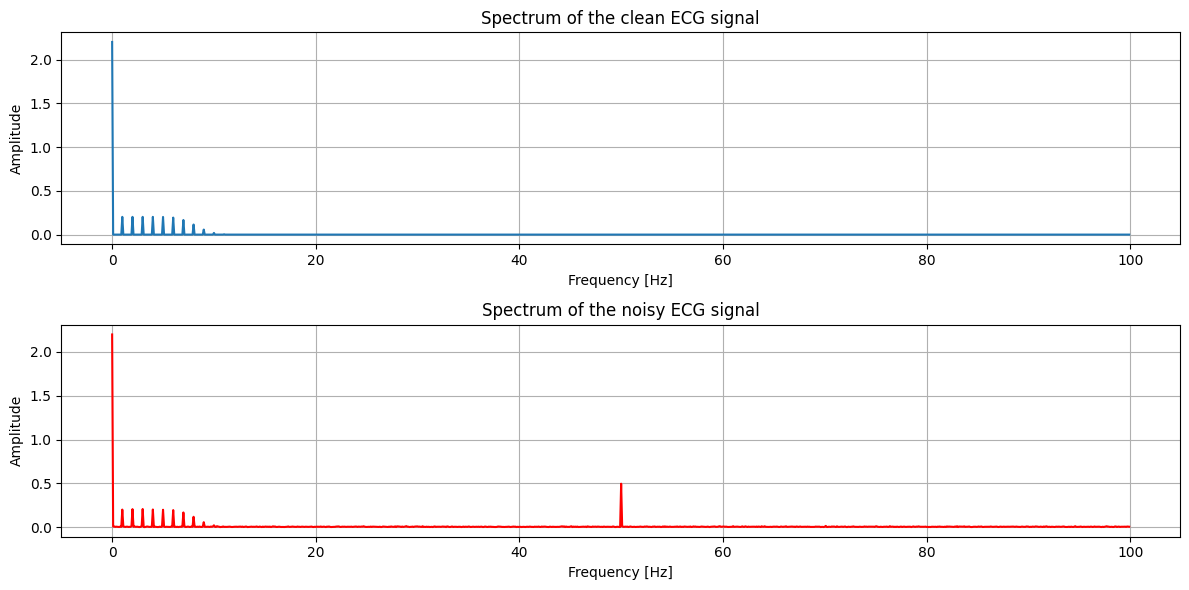
\includegraphics[width=0.9\textwidth]{./figures/ecg_spectra.png}
    \caption{Spectrum of the Clean ECG Signal (Top) and Noisy ECG Signal (Bottom)}
\end{figure}

\textbf{Observations:}
	\begin{itemize}
		\item In the clean ECG spectrum, the main frequency components correspond to the heart rate and its harmonics.
		\item In the noisy ECG spectrum, there is a prominent peak at 50 Hz due to the power line interference.
		\item The noise introduces additional frequency components, increasing the overall noise floor in the spectrum.
	\end{itemize}
\textbf{Conclusions:}
	\begin{itemize}
		\item The 50 Hz interference is clearly visible in the noisy signal's spectrum, which can be targeted for filtering.
		\item The random noise raises the baseline of the spectrum, indicating increased noise across all frequencies.
	\end{itemize}

\subsection{Normalize the signal from -1 to 1. Plot the original and quantized signal for 2, 4, and 8 bits (there are 3 graphs). What do you observe in the graphs?}

\subsubsection*{Code for Normalization and Quantization}

\begin{lstlisting}[language=Python]
# Normalize the signal from -1 to 1
ecg_normalized = 2 * (ecg_sampled - np.min(ecg_sampled)) / (np.max(ecg_sampled) - np.min(ecg_sampled)) - 1

def cuantizar(s, bit):
    # s: input signal normalized between -1 and 1
    # bit: number of quantization bits
    levels = 2 ** bit
    s_quantized = np.round(((s + 1) / 2) * (levels - 1))  # Scale and quantize
    s_quantized = s_quantized / (levels - 1) * 2 - 1  # Scale back to -1 and 1
    return s_quantized

# Quantization
ecg_quantized_2bit = cuantizar(ecg_normalized, 2)
ecg_quantized_4bit = cuantizar(ecg_normalized, 4)
ecg_quantized_8bit = cuantizar(ecg_normalized, 8)

# Select a segment to plot
start_sample = 950
end_sample = 1150
time_segment = time[start_sample:end_sample]

# Plot for 2 bits
plt.figure(figsize=(10, 4))
plt.plot(time_segment, ecg_normalized[start_sample:end_sample], label='Original', alpha=0.7)
plt.step(time_segment, ecg_quantized_2bit[start_sample:end_sample], label='Quantized (2 bits)', where='mid')
plt.title('Original Signal vs Quantized (2 bits)')
plt.xlabel('Time [s]')
plt.ylabel('Amplitude')
plt.legend()
plt.grid()
plt.show()

# Plot for 4 bits
plt.figure(figsize=(10, 4))
plt.plot(time_segment, ecg_normalized[start_sample:end_sample], label='Original', alpha=0.7)
plt.step(time_segment, ecg_quantized_4bit[start_sample:end_sample], label='Quantized (4 bits)', where='mid')
plt.title('Original Signal vs Quantized (4 bits)')
plt.xlabel('Time [s]')
plt.ylabel('Amplitude')
plt.legend()
plt.grid()
plt.show()

# Plot for 8 bits
plt.figure(figsize=(10, 4))
plt.plot(time_segment, ecg_normalized[start_sample:end_sample], label='Original', alpha=0.7)
plt.step(time_segment, ecg_quantized_8bit[start_sample:end_sample], label='Quantized (8 bits)', where='mid')
plt.title('Original Signal vs Quantized (8 bits)')
plt.xlabel('Time [s]')
plt.ylabel('Amplitude')
plt.legend()
plt.grid()
plt.show()
\end{lstlisting}

\subsubsection*{Results and Discussion}

\textbf{Quantization with 2 Bits:}

\begin{figure}[H]
    \centering
    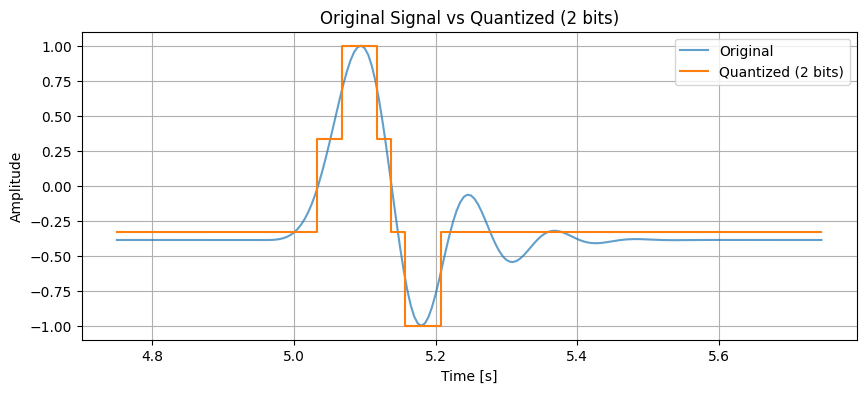
\includegraphics[width=0.8\textwidth]{./figures/ecg_quantized_2bit.png}
    \caption{Original vs Quantized ECG Signal (2 bits)}
\end{figure}

\textbf{Quantization with 4 Bits:}

\begin{figure}[H]
    \centering
    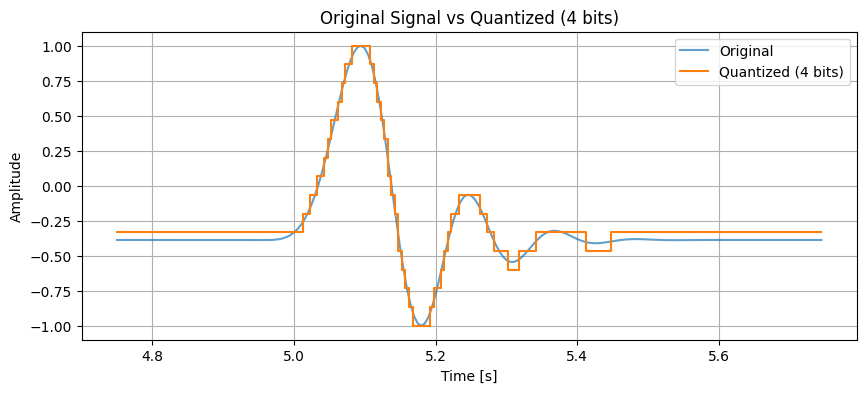
\includegraphics[width=0.8\textwidth]{./figures/ecg_quantized_4bit.png}
    \caption{Original vs Quantized ECG Signal (4 bits)}
\end{figure}

\textbf{Quantization with 8 Bits:}

\begin{figure}[H]
    \centering
    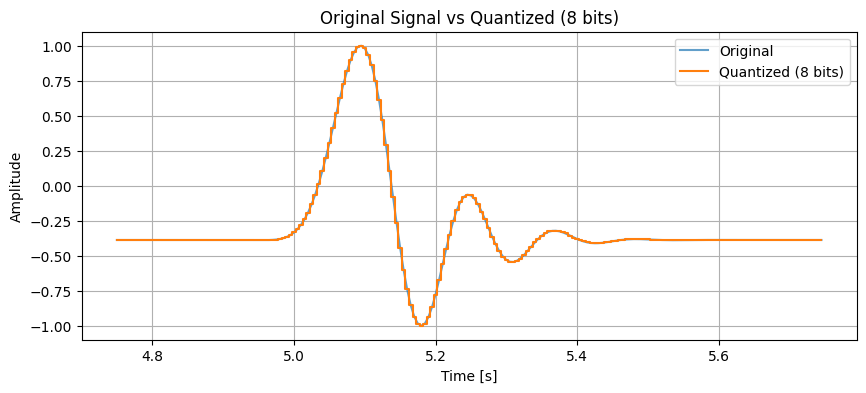
\includegraphics[width=0.8\textwidth]{./figures/ecg_quantized_8bit.png}
    \caption{Original vs Quantized ECG Signal (8 bits)}
\end{figure}

\textbf{Observations:}

\begin{itemize}
	\item \textbf{2 Bits:} The quantized signal appears as a coarse approximation of the original signal with only 4 quantization levels. The waveform is heavily distorted, and fine details are lost.
	\item \textbf{4 Bits:} With 16 quantization levels, the quantized signal follows the original signal more closely. However, there are still noticeable steps in the waveform.
	\item \textbf{8 Bits:} The quantized signal closely matches the original signal. The increased number of levels (256) allows for a much finer representation, and the steps are barely perceptible.
\end{itemize}

\textbf{Conclusions:}

\begin{itemize}
	\item Increasing the number of quantization bits improves the fidelity of the quantized signal.
	\item At lower bit depths, quantization error is significant, leading to distortion of the signal.
	\item For applications requiring high accuracy, a higher bit depth is necessary to preserve the integrity of the ECG signal.
\end{itemize}

\subsection{Overall Conclusions}

\begin{itemize}
	\item The presence of noise, especially the 50 Hz interference, significantly affects the quality of the ECG signal.
	\item Frequency analysis using FFT allows us to identify and potentially filter out unwanted frequency components.
	\item Quantization introduces errors that depend on the number of bits used. Adequate bit depth is essential for accurate signal representation in digital systems.
\end{itemize}



\end{document}